% European Journal of Physics -- Paper (Mechanics), students' computational project
%
% Build:  pdflatex manuscript && bibtex manuscript && pdflatex manuscript && pdflatex manuscript
%
% EJP asks for a single PDF at first submission with figures in place and type
% no smaller than 12 pt. Its LaTeX template is optional and is not used here.
\documentclass[12pt,a4paper]{article}
\usepackage[margin=2.5cm]{geometry}
\usepackage[T1]{fontenc}
\usepackage{lmodern}
\usepackage{amsmath,amssymb,bm}
\usepackage{graphicx}
\usepackage{booktabs}
\usepackage{setspace}
\usepackage[numbers,sort&compress]{natbib}
\usepackage[hidelinks]{hyperref}
\graphicspath{{../figures/}}
% Generated by code/analysis.py from data/summary.json. Do not edit by hand.
\newcommand{\secPerUnit}{0.319}
\newcommand{\lamBen}{0.299}
\newcommand{\lamBenEns}{0.296}
\newcommand{\nEns}{47}
\newcommand{\nChaotic}{44}
\newcommand{\nReg}{3}
\newcommand{\lamDir}{0.33}
\newcommand{\lamDirEarly}{0.28}
\newcommand{\lamDirLate}{0.33}
\newcommand{\lamDirOther}{0.329}
\newcommand{\slopeStep}{7.9}
\newcommand{\slopeStepSE}{0.4}
\newcommand{\slopeStepPred}{9.3}
\newcommand{\lamStep}{0.35}
\newcommand{\lamStepSE}{0.02}
\newcommand{\slopePrec}{1.99}
\newcommand{\slopePrecSE}{0.06}
\newcommand{\slopePrecPred}{2.32}
\newcommand{\lamPrec}{0.35}
\newcommand{\lamPrecSE}{0.01}
\newcommand{\gammaRound}{0.6}
\newcommand{\gammaLo}{0.3}
\newcommand{\gammaHi}{0.8}
\newcommand{\lamDirWin}{0.35}
\newcommand{\lamPrecCoarse}{0.31}
\newcommand{\lamPrecFine}{0.34}
\newcommand{\lamExcess}{18}
\newcommand{\TsingleFine}{30}
\newcommand{\collapseSpan}{8}
\newcommand{\collapse}{0.21}
\newcommand{\rkOrder}{4.000}
\newcommand{\ordEuler}{1.002}
\newcommand{\ordMid}{1.999}
\newcommand{\TEulerFine}{31}
\newcommand{\TRKcoarse}{43}
\newcommand{\TkEight}{79}
\newcommand{\TkEleven}{97}
\newcommand{\TBestDouble}{101}
\newcommand{\TBestDoubleSec}{32}
\newcommand{\kBestDouble}{11}
\newcommand{\TBestSingle}{53}
\newcommand{\TBestSingleSec}{17}
\newcommand{\kBestSingle}{7}
\newcommand{\kRatio}{64}
\newcommand{\TdoubleFine}{98}
\newcommand{\TdoubleKten}{92}
\newcommand{\dEexp}{10}
\newcommand{\costFactor}{2000}
\newcommand{\extraBits}{50}
\newcommand{\lamSI}{0.94}
\newcommand{\decadeSI}{10}
\newcommand{\bestRows}{24 (single) & $2^{-7}$ & 53 & 17 \\
32 & $2^{-7}$ & 66 & 21 \\
40 & $2^{-9}$ & 79 & 25 \\
53 (double) & $2^{-11}$ & 101 & 32 \\
64 (extended) & $2^{-15}$ & 124 & 40 \\}

\onehalfspacing

\title{Step size, floating-point precision and the predictability horizon of a
simulated double pendulum: a student computational project}
\author{Luke Wang and Arjun Pemmasani\\[4pt]
\small Harvey Mudd College, Claremont, CA 91711, United States of America\\
\small E-mail: \texttt{arjun.pemmasani@gmail.com}}
\date{}

\begin{document}
\maketitle

\begin{abstract}
\noindent We report a computational project, begun in an undergraduate course in
numerical analysis, on a question that students who simulate chaotic systems
rarely put to their own programs: for how long is the computed trajectory the
right one? The double pendulum is integrated with a fixed-step fourth-order
Runge--Kutta method in arbitrary-precision arithmetic, which allows the step $h$
and the number of significand bits $p$ to be varied independently and the
effects of truncation and of roundoff to be measured separately. The time $T$ for
which a run agrees with a far more accurate reference obeys a single law
governed by the largest Lyapunov exponent $\lambda$: each halving of $h$ extends
$T$ by $4\ln2/\lambda$, each additional bit extends it by $\ln2/\lambda$, and for
any given precision there is a best step beyond which refinement shortens $T$.
The slopes yield $\lambda=\lamStep\pm\lamStepSE$ and $\lamPrec\pm\lamPrecSE$, equal to the
growth rate of a perturbed trajectory over the same interval and within 20\% of
the long-time exponent \lamBen\ from the standard two-trajectory method. In double precision the
pendulum cannot be followed for more than about \TBestDouble\ natural time units
with this method, while its energy stays constant to a part in $10^{\dEexp}$
throughout. The project is suitable for advanced undergraduates in physics or
applied mathematics, requires only a short program, and shows numerical error to
be a perturbation like any other, one whose growth measures the dynamics.
\end{abstract}

\noindent\textbf{Keywords:} double pendulum, chaos, Lyapunov exponent, numerical
integration, roundoff error, computational physics education

\section{Introduction}

The double pendulum is among the simplest mechanical systems that are chaotic,
and it is correspondingly popular in teaching. In this journal
D'Alessio~\cite{dalessio2023} has given a combined analytical, numerical and
experimental treatment, including the full spectrum of Lyapunov exponents, aimed
at upper-year undergraduates. Earlier pedagogical studies measured the divergence
of two real pendulums released together~\cite{shinbrot1992}, developed the
apparatus as a laboratory experiment~\cite{levien1993}, and mapped the onset of
chaos numerically as a function of energy~\cite{stachowiak2006}. In all of them
the simulation is a tool, and its output is taken to be the motion of the
pendulum.

This paper is about the tool. Sensitive dependence on initial conditions means
that a small perturbation grows exponentially, and a numerical integrator
supplies a small perturbation at every step, by truncating the Taylor series of
the solution and by rounding each arithmetic result. The computed trajectory must
therefore leave the true one after a finite time, however carefully the program
is written. Lorenz~\cite{lorenz1963} met chaos in precisely this way, and
Lighthill~\cite{lighthill1986} later called the time in question the horizon of
predictability. The reliability of long computations of chaotic systems has since
been examined in atmospheric modelling~\cite{teixeira2007} and with
multiple-precision arithmetic~\cite{liao2009}. Yet in our experience students who
simulate a double pendulum are seldom asked how long their result can be
believed, and the informal checks they apply, such as watching the energy, cannot
tell them.

The work described here began as our final project in an undergraduate course
on numerical analysis. We simulated identical double pendulums with
different steps and different floating-point formats and watched the
trajectories separate. The observation that prompted this paper was that a step
ten times smaller, at ten times the cost, bought only five to ten more seconds
of agreement. Here we redo the project with a cleaner design, explain that
observation, and show that the explanation is quantitative: the numerical error
measures the Lyapunov exponent.

We believe the project is useful to physics education at the advanced
undergraduate level in three ways. It gives students a concrete meaning for the
Lyapunov exponent in terms of something they control. It separates truncation
error from roundoff error, which are usually taught together and rarely
distinguished in practice. And it corrects two common beliefs: that a smaller
step always gives a better answer, and that conservation of energy certifies a
trajectory.

\section{The project}

\subsection{Model}

Two point masses $m$ are suspended in series from a fixed pivot by massless rigid
rods of length $l$ and move in a vertical plane. The angles $\theta_1$ and
$\theta_2$ are measured from the downward vertical. Measuring time in units of
$\sqrt{l/g}$ removes every parameter from the Lagrangian equations of motion,
which become
\begin{align}
\ddot\theta_1 &= \frac{\omega_1^2\sin\Delta\cos\Delta+\sin\theta_2\cos\Delta
                +\omega_2^2\sin\Delta-2\sin\theta_1}{2-\cos^2\Delta},\label{eq:eom1}\\
\ddot\theta_2 &= \frac{-\omega_2^2\sin\Delta\cos\Delta
                +2\left(\sin\theta_1\cos\Delta-\omega_1^2\sin\Delta-\sin\theta_2\right)}
                {2-\cos^2\Delta},\label{eq:eom2}
\end{align}
with $\omega_i=\dot\theta_i$ and $\Delta=\theta_2-\theta_1$. The conserved energy
in units of $mgl$ is
\begin{equation}
E=\omega_1^2+\tfrac12\omega_2^2+\omega_1\omega_2\cos\Delta-2\cos\theta_1-\cos\theta_2 .
\end{equation}
The pendulum is released from rest with both rods horizontal, so that $E=0$. For
$l=1$~m one time unit is \secPerUnit~s.

\subsection{Numerical method}

Equations (\ref{eq:eom1}) and (\ref{eq:eom2}) are written as a first-order system
for $\bm y=(\theta_1,\theta_2,\omega_1,\omega_2)$ and advanced with the classical
fourth-order Runge--Kutta method (RK4)~\cite{hairer1993} at a fixed step $h$. We
avoid adaptive step-size control deliberately, since its purpose is to hide the
dependence on $h$ that we want to see.

The arithmetic is done by the MPFR library~\cite{fousse2007}, which rounds each
operation correctly to a significand of $p$ bits, where $p$ is set by the
program. Our first version used Julia's \texttt{BigFloat} type and the present
one uses Python with \texttt{gmpy2}; both are thin wrappers around MPFR. With
$p=24$, 53, 64 and 113 the significand has the width of the IEEE single, double,
extended and quadruple formats~\cite{goldberg1991}. With $p=237$, the width of
the 256-bit format, the rounding unit is $10^{-71}$ and the arithmetic is exact
for our purposes.

One detail of design proved important. Our first version used decimal steps such
as $h=10^{-4}$. No binary format represents $10^{-4}$ exactly, so runs at
different precisions were also using slightly different steps. We now take
$h=2^{-k}$, which is exact at every precision, and changing $p$ then changes the
arithmetic and nothing else.

\subsection{Measuring error without an exact solution}

We measure the error of a run by the distance $d(t)$, in units of $l$, between
its lower bob and that of a reference run. Because both bobs lie within $2l$ of
the pivot, $d$ saturates near 4 when two runs have become unrelated. The
\emph{horizon} $T$ of a run is the first time at which $d\ge10^{-2}$, which is
about when two superimposed animations can be told apart by eye.

The reference is simply a run that is much more accurate, and an elementary
argument says how far it can be trusted. If $e_a$ and $e_r$ are the true errors
of a run and of the reference, the triangle inequality gives $|d-e_a|\le e_r$.
Both errors are amplified by the same dynamics, so their ratio stays near its
initial value, which for RK4 runs with steps $2^{-k_a}$ and $2^{-k_r}$ is
$2^{-4(k_r-k_a)}$. With $k_r=18$, the separation $d$ equals the true error of
every run with $k_a\le16$ to better than half a per cent, until that run reaches
its own horizon.

\subsection{Three experiments}

\begin{description}
\item[Truncation only.] With $p=237$, vary $k$ from 4 to 17 and compare with
$k=18$. Roundoff is fifty orders of magnitude below truncation.
\item[Roundoff only.] With $h$ fixed, vary $p$ from 11 to 128 and compare with
the run at $p=237$ and the \emph{same} $h$. The two runs iterate the same discrete
map, so their truncation errors are identical and cancel. What remains is
rounding. Ordinary hardware arithmetic offers no way of making this separation.
\item[Both.] With $p=24$, 32, 40, 53 and 64, vary $k$ and compare with the
reference of the first experiment. This is the position of a student using
single or double precision.
\end{description}

\section{A model for the horizon}
\label{sec:model}

Let $\bm e_n$ be the error after $n$ steps. One further step gives
$\bm e_{n+1}=\mathsf J_n\bm e_n+\bm\tau_n+\bm\rho_n$, in which $\mathsf J_n$ is
the Jacobian of the flow over the step, $\bm\tau_n=O(h^5)$ is the local truncation
error and $\bm\rho_n=O(2^{-p})$ the rounding error. The error at time $t$ is thus
a sum over earlier steps of the error committed at each, propagated by the
product of the Jacobians in between. For a chaotic trajectory that product grows
on average as $e^{\lambda(t-t_j)}$, with $\lambda$ the largest Lyapunov exponent,
and the sum is dominated by its earliest terms:
\begin{equation}
e(t)\approx\left(A\,h^{4}+B\,2^{-p}h^{-\gamma}\right)e^{\lambda t}.
\label{eq:error}
\end{equation}
The first term comes from $1/h$ truncation errors of size $h^5$ per unit time. The
second comes from $1/h$ rounding errors of size $2^{-p}$ per unit time, with
$\gamma=\tfrac12$ if they accumulate as a random walk and $\gamma=1$ if they
accumulate systematically~\cite{hairer2008}. Setting $e(T)=\epsilon$ gives
\begin{equation}
T=\frac1\lambda\ln\frac{\epsilon}{A\,h^{4}+B\,2^{-p}h^{-\gamma}} .
\label{eq:horizon}
\end{equation}
With $h=2^{-k}$ the two limiting cases are
\begin{align}
T&=T_A+\frac{4\ln2}{\lambda}\,k &&\text{(truncation dominant)},\label{eq:Tk}\\
T&=T_B+\frac{\ln2}{\lambda}\,(p-\gamma k) &&\text{(roundoff dominant)}.\label{eq:Tp}
\end{align}
Halving the step extends the horizon by a fixed amount when truncation dominates
and shortens it when roundoff does; each extra bit extends it by a fixed amount.
The regimes meet at $k^\ast=[p+\log_2(A/B)]/(4+\gamma)$, where the horizon takes
its greatest value for that precision,
$T_{\max}\approx\mathrm{const}+(\ln2/\lambda)\,4p/(4+\gamma)$. The only property
of the pendulum in any of these slopes is $\lambda$.

\section{Results}

\subsection{Step size}

Figure~\ref{fig:snap} shows three pendulums that differ only in step. They are
indistinguishable for tens of time units and then separate one at a time, largest
step first. Figure~\ref{fig:step}(a) shows the corresponding errors. They rise at
a common average rate over many orders of magnitude, and they are evenly spaced
because, as figure~\ref{fig:step}(b) shows, they are the same curve scaled by
$h^4$: multiplied by $h^{-4}$ they coincide to within \collapse\ decades for
every $h\le2^{-8}$ wherever none has saturated. The error at $t=10$ scales as
$h^{\rkOrder}$.

\begin{figure}[t]
\centering
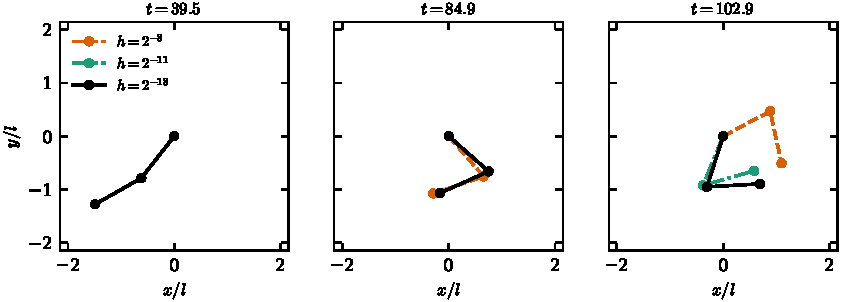
\includegraphics[width=\textwidth]{fig1_snapshots}
\caption{Three double pendulums released from the same state and integrated with
the same 237-bit arithmetic, differing only in step $h$. The run with
$h=2^{-8}$ departs near $t=\TkEight$ and the run with $h=2^{-11}$ near
$t=\TkEleven$ (time in units of $\sqrt{l/g}$). An animation is provided as
supplementary material.}
\label{fig:snap}
\end{figure}

\begin{figure}[t]
\centering
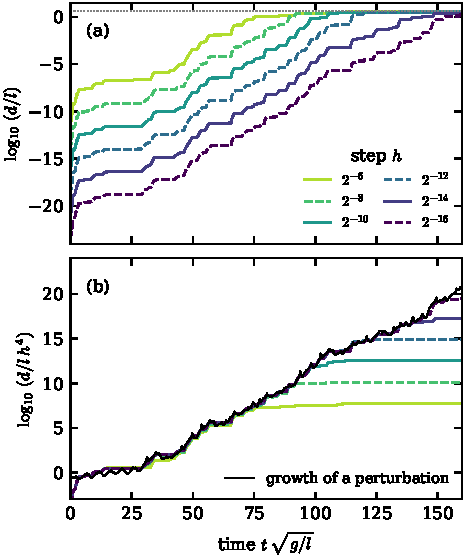
\includegraphics[width=0.62\textwidth]{fig2_step_sweep}
\caption{(a) Separation $d$ of the lower bob from that of the reference
($h=2^{-18}$) in 237-bit arithmetic (running maximum). The dotted line is the
largest possible separation. (b) The same curves multiplied by $h^{-4}$. The thin
black line is the separation of two runs whose initial conditions differ by
$2^{-170}$, shifted vertically.}
\label{fig:step}
\end{figure}

The common curve is the amplification factor of the trajectory. To check this we
perturbed $\theta_1(0)$ by $2^{-170}$, which is small enough to stay in the linear
regime for the whole run, and the resulting separation, drawn as the thin line
in figure~\ref{fig:step}(b), follows the collapsed error curves through every
plateau and burst. The integrator's error grows as a perturbation of the initial
condition grows because that is what it is. The growth is exponential only on
average; the local rate varies as the pendulum visits more and less unstable
configurations.

Figure~\ref{fig:hor}(a) shows the horizon against $k$. A line fitted over
$7\le k\le16$ has slope $\slopeStep\pm\slopeStepSE$ time units per halving, and
equation~(\ref{eq:Tk}) gives $\lambda=\lamStep\pm\lamStepSE$. The scatter about the
line is real. A horizon that falls just before a burst of growth gains little
from the next halving, and one that falls just after gains a great deal. The
grey staircase in figure~\ref{fig:hor}(a) is the horizon predicted for every $h$
from the measured growth of the $2^{-170}$ perturbation, with the one constant
$A$ of equation~(\ref{eq:error}) fixed by the collapse. It passes through the
measured horizons step for step.

\begin{figure}[t]
\centering
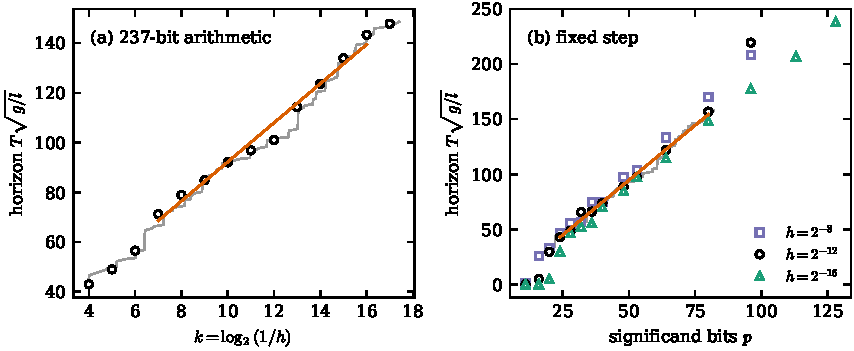
\includegraphics[width=\textwidth]{fig4_horizons}
\caption{Horizon $T$, the first time at which $d\ge10^{-2}$. (a) Against
$k=\log_2(1/h)$ in 237-bit arithmetic: truncation only. (b) Against the number of
significand bits $p$ at fixed step: roundoff only. The straight lines are
least-squares fits whose slopes give $\lambda$ through equations (\ref{eq:Tk}) and
(\ref{eq:Tp}). The grey staircases are the horizons predicted from the measured
growth of a perturbation of the initial condition.}
\label{fig:hor}
\end{figure}

\subsection{Precision}

Figure~\ref{fig:prec} shows the second experiment at $h=2^{-12}$. The pattern is
that of figure~\ref{fig:step} with $2^{-p}$ in the place of $h^4$. The horizons in
figure~\ref{fig:hor}(b) have slope $\slopePrec\pm\slopePrecSE$ time units per bit,
so that $\lambda=\lamPrec\pm\lamPrecSE$ from equation~(\ref{eq:Tp}). Changing the
step by a factor of 256 shifts the line only slightly. Comparing errors at fixed
early times for $h=2^{-8}$ and $2^{-16}$ gives $\gamma\approx\gammaRound$, between
the random-walk and the systematic limits.

\begin{figure}[t]
\centering
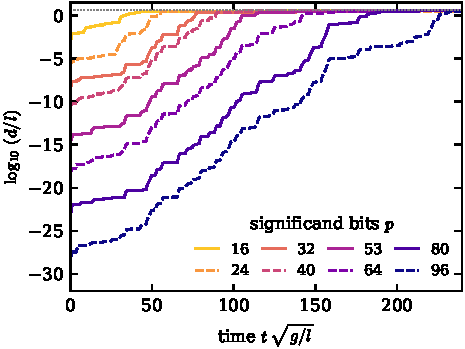
\includegraphics[width=0.62\textwidth]{fig3_precision_sweep}
\caption{Separation from the 237-bit run at the same step, $h=2^{-12}$, for eight
significand widths. Truncation error is common to each pair and cancels, so that
only roundoff is seen.}
\label{fig:prec}
\end{figure}

The lowest precisions were left out of the fit, and the reason was the most
memorable moment of the project. With $p=11$ and $h=2^{-12}$ the pendulum never
moves. The first increment to $\theta_1=\pi/2$ is less than half a unit in the
last of eleven bits, the sum rounds back to $\pi/2$, and the pendulum hangs
horizontally for ever. With the same eleven bits and $h=2^{-8}$ it falls. A
smaller step has made the error total.

\subsection{The Lyapunov exponent four ways}

Table~\ref{tab:lambda} compares the estimates. The conventional value is from the
two-trajectory method of Benettin \textit{et al}~\cite{benettin1980a,benettin1980b,wolf1985}:
a shadow orbit at distance $10^{-8}$ is advanced with the fiducial orbit, and once
per time unit the logarithm of the growth of their separation is accumulated and
the shadow is returned to its original distance. Over $2\times10^4$ time units
this gives $\lambda=\lamBen$. Of \nEns\ other states at rest with the same energy,
\nChaotic\ are chaotic with median \lamBenEns, and \nReg\ lie on regular orbits.
The direct growth rate of the $2^{-170}$ perturbation is \lamDir\ over the whole
run and \lamDirWin\ for $t>20$, after the slow start from rest.

The two values obtained from numerical error agree with each other and with the
direct growth rate over the same interval. All three exceed the long-time value
by some \lamExcess\%. This is not a failure of the method. A horizon samples the
growth rate only up to the horizon, and over its first 160 time units this
trajectory is more unstable than it is on average. The exponent proper is a
long-time limit about which finite-time values scatter, a distinction that
students who picture exponential divergence as uniform do well to meet.

\begin{table}[t]
\centering
\caption{Largest Lyapunov exponent for release from rest with both rods
horizontal, in units of $\sqrt{g/l}$. The last three rows sample only the first
160 time units, over which the mean growth rate is \lamDirEarly\ in the first half
and \lamDirLate\ in the second. Uncertainties are standard errors of the fitted
slopes. At $h=2^{-8}$ and $2^{-16}$ the last row becomes \lamPrecCoarse\ and
\lamPrecFine.}
\label{tab:lambda}
\begin{tabular}{lc}
\toprule
Method & $\lambda$\\
\midrule
Two-trajectory method, $2\times10^4$ time units & \lamBen\\
Growth of a $2^{-170}$ perturbation & \lamDir\\
Horizon against step, equation (\ref{eq:Tk}) & $\lamStep\pm\lamStepSE$\\
Horizon against precision, equation (\ref{eq:Tp}) & $\lamPrec\pm\lamPrecSE$\\
\bottomrule
\end{tabular}
\end{table}

\subsection{Working precision}

Figure~\ref{fig:turn} shows the third experiment. At large steps all precisions
agree, since truncation dominates. As the step is reduced each curve leaves the
237-bit line in turn and flattens, and at the lower precisions it then falls, as
equation~(\ref{eq:horizon}) predicts. Table~\ref{tab:best} lists the best step and the longest horizon for
each. In double precision the longest horizon is \TBestDouble\ time units,
\TBestDoubleSec~s for one-metre rods, reached at $h=2^{-\kBestDouble}$. Reducing the
step further to $2^{-17}$ costs \kRatio\ times as much and gives \TdoubleFine. In
single precision the best horizon is \TBestSingle, at $h=2^{-\kBestSingle}$, and
by $h=2^{-17}$ it has fallen to \TsingleFine.

\begin{figure}[t]
\centering
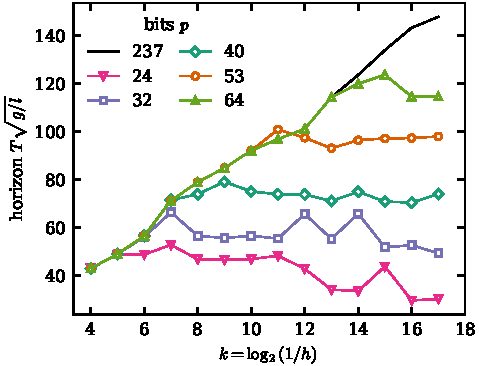
\includegraphics[width=0.62\textwidth]{fig5_turnover}
\caption{Horizon against step for five working precisions, with the 237-bit
result for comparison. Each precision has a step beyond which refinement no
longer helps.}
\label{fig:turn}
\end{figure}

\begin{table}[t]
\centering
\caption{Longest horizon attainable with RK4 at each precision. The last column
is for $l=1$~m.}
\label{tab:best}
\begin{tabular}{lccc}
\toprule
Significand bits $p$ & Best step & $T_{\max}\sqrt{g/l}$ & $T_{\max}$ (s)\\
\midrule
\bestRows
\bottomrule
\end{tabular}
\end{table}

\subsection{Energy}

Figure~\ref{fig:energy} shows both errors for an ordinary double-precision run
with $h=2^{-10}$. The energy error drifts slowly upward, as expected of a
non-symplectic method, and never exceeds $10^{-\dEexp}$. The trajectory is lost at
$t\approx\TdoubleKten$. Energy confines the state to a three-dimensional surface
in phase space, and chaotic divergence takes place within that surface, so that a
computed state can wander arbitrarily far along it without leaving it.

\begin{figure}[t]
\centering
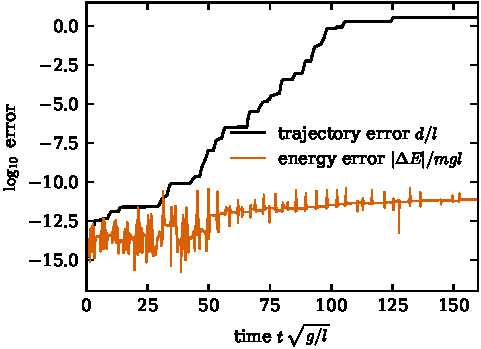
\includegraphics[width=0.62\textwidth]{fig6_energy}
\caption{Error in the position of the lower bob and in the energy for a run in
double precision with $h=2^{-10}$.}
\label{fig:energy}
\end{figure}

\section{Discussion}

\subsection{The price of a longer horizon}

The work of a fixed-step run is proportional to $2^k$. From
equation~(\ref{eq:Tk}), a gain of $\Delta T$ needs
$\Delta k=\lambda\Delta T/(4\ln2)$ and multiplies the work by
$e^{\lambda\Delta T/4}$, and the precision must rise by about
$\lambda\Delta T(4+\gamma)/(4\ln2)$ bits to stay at the optimum. Doubling the
double-precision horizon of this pendulum would multiply the number of steps by
about \costFactor\ and need some \extraBits\ more bits. The horizon grows as the
logarithm of the effort. In everyday units, $\lambda=\lamSI$~s$^{-1}$ for
one-metre rods, and a tenfold reduction of the step buys
$4\ln10/\lambda\approx\decadeSI$~s, which is what we saw in our first crude runs.

A method of order $n$ replaces 4 by $n$. We verified that the error of forward
Euler at fixed time scales as $h^{\ordEuler}$ and that of the explicit midpoint
rule as $h^{\ordMid}$. Forward Euler with $h=2^{-16}$ has a horizon of
\TEulerFine\ time units, shorter than the \TRKcoarse\ of RK4 with $h=2^{-4}$. For
chaotic problems the case for high-order methods is stronger than usual.

\subsection{What survives the horizon}

After $T$ the computed trajectory is no longer the solution of the problem
posed, but shadowing results~\cite{hammel1987,hammel1988,grebogi1990,sauer1997}
show that for long times it stays close to an exact trajectory with slightly
different initial data. Averages over the motion are therefore still computed
correctly. As a check we computed the time-averaged kinetic energy over $10^4$
time units in single and in double precision and found 1.357 and 1.358, although
the two trajectories part after about fifty time units. The first row of
table~\ref{tab:lambda} relies on the same fact.

\subsection{Running the project with a class}

The program is the usual RK4 with the number type changed, and apart from the two
finest reference runs everything reported here finishes in minutes on a laptop.
The natural sequence is the one we followed. Students first overlay animations
of runs that differ in step or precision and see them separate. They then plot
the separation on a logarithmic scale and find straight lines, fit the horizons,
and compare the resulting $\lambda$ with a two-trajectory estimate. Students
without a multiple-precision library can still carry out the third experiment,
using double precision at the best step of table~\ref{tab:best} as the reference
for single precision. Natural extensions are other energies, where $\lambda$ is
smaller and some orbits are regular, so that the error grows only as a power of
$t$; a symplectic integrator, to find out whether preserving phase-space
structure helps with prediction; and other chaotic systems, such as the Lorenz
equations, for which the double-precision horizon can be predicted from the known
exponent before it is measured.

\section{Conclusion}

A simulation of a chaotic system is accurate for a time that depends
logarithmically on the error committed per step. For the double pendulum
integrated by RK4 that time increases by $4\ln2/\lambda$ per halving of the step
and by $\ln2/\lambda$ per bit of precision, up to a ceiling set by whichever
source of error is larger, and in double precision the ceiling is about
\TBestDouble\ natural time units. The same measurements give the finite-time Lyapunov exponent of the trajectory
to within a few per cent, and its long-time value to within twenty. Students who complete the project come to
see truncation and roundoff as perturbations to which the system responds as it
does to any other, and they learn to ask of any simulation how long it has been
right.

\section*{Acknowledgments}
This work began as a final project in Math~165, Numerical Analysis, at Harvey
Mudd College.

\section*{Data availability statement}
The code that produced every result and figure, the numerical data plotted, and
two animations are provided as supplementary material.

\section*{Conflict of interest}
The authors declare no conflict of interest.

\bibliographystyle{unsrtnat}
\bibliography{../refs}

\end{document}
